\chapter{Tinjauan Pustaka}

% Daftar keterangan variabel yang dipasang di bawah setiap persamaan.
\newenvironment{keterangan}{%
  \par\vspace{3pt}\noindent dengan:\par\nobreak
  % leftmargin = labelwidth + labelsep agar baris sambungan rata dengan
  % baris pertama keterangan, bukan menjorok lebih dalam.
  \begin{description}[leftmargin=2.8cm,labelwidth=2.4cm,labelsep=0.4cm,
    align=left,font=\normalfont,topsep=2pt,itemsep=0pt,parsep=0pt]%
}{%
  \end{description}\par\vspace{3pt}%
}

\section{Penelitian Terdahulu}
Penelitian terdahulu yang relevan dikelompokkan ke dalam empat kelompok:
perbandingan model ML dengan HAR untuk volatilitas aset kripto, uji
instabilitas peramalan pada aset kripto, pengaruh \textit{window} data latih,
serta evolusi karakteristik pasar Bitcoin.

\textbf{Perbandingan ML dan HAR untuk volatilitas kripto.} Dudek dkk.
merupakan paper acuan penelitian ini. Penelitian tersebut membandingkan sejumlah
model untuk volatilitas kripto pada periode 2019--2021 dengan satu skema
\textit{rolling window} sepanjang 23 bulan dan pelatihan ulang harian, lalu
melaporkan kinerja sebagai satu angka agregat \cite{dudek2024}. Kinerja pada
5\% hari dengan RV terendah dan tertinggi dibandingkan secara deskriptif tanpa
uji formal, dan model berbasis pohon, khususnya Random Forest, termasuk yang
terburuk ketika volatilitas tinggi. Huang, Sangiorgi, dan Urquhart menemukan
bahwa LSTM unggul tipis atas HAR, sekitar 1,56\% dengan masukan setara, pada
periode \textit{out-of-sample} sekitar 290 hari, sedangkan HAR lebih baik ketika
terjadi lonjakan volatilitas \cite{huang2024}. Wang, Andreeva, dan
Martin-Barragan menunjukkan bahwa prediktor internal pasar merupakan prediktor
terpenting \cite{wang2023}, berbeda dengan Feng, Qi, dan Lucey yang menemukan
bahwa kepentingan fitur berubah sejak Oktober 2022 dan yang memvariasikan
\textit{hyperparameter} model secara harian \cite{feng2024ml}. Qiu dkk.
menunjukkan bahwa spesifikasi model yang tetap tidak berlaku universal
\cite{qiu2025}. Oprea dan Bâra mengkaji peran \textit{regime} tetapi
menargetkan harga, bukan volatilitas, dan tanpa HAR sebagai pembanding
\cite{oprea2026}.

% CEK: Feng, Qi & Lucey (2024) baru abstrak; Qiu dkk. (2025) baru metadata.

\textbf{Uji instabilitas peramalan pada aset kripto.} Trucíos dan Taylor
menerapkan \textit{Fluctuation test} pada peramalan \textit{Value at Risk} dan
\textit{Expected Shortfall} aset kripto menggunakan model ekonometrik
\cite{trucios2023}. Penelitian tersebut menunjukkan bahwa alat uji instabilitas
relevan untuk aset kripto, tetapi tidak mencakup model ML maupun target RV.

\textbf{Pengaruh \textit{window} data latih.} Akgun dan Gulay membandingkan
sebelas model tipe GARCH dan tiga model \textit{deep learning} untuk peramalan
volatilitas Bitcoin, Ethereum, dan Binance Coin hingga akhir 2021
\cite{akgun2025}. Perbandingan \textit{rolling} dan \textit{expanding window}
dilaporkan secara rinci untuk model tipe GARCH, dengan hasil bahwa
\textit{rolling window} umumnya lebih akurat; perbandingan tersebut tidak
menyertakan HAR dan tidak disertai uji signifikansi. Chassot dan Audrino menunjukkan pada 1.445 saham bahwa model
ML gagal mengalahkan HAR ketika HAR diberi skema \textit{fitting} yang tepat
\cite{chassot2026}, sehingga keunggulan ML yang dilaporkan dapat merupakan
artefak perlakuan \textit{window} yang tidak setara.

\textbf{Evolusi pasar Bitcoin dan peran \textit{regime}.} Do menetapkan
pembagian era pasar Bitcoin dan menunjukkan perubahan persistensi RV serta
hubungan volatilitas--likuiditas antarera \cite{do2026}. Mokni dkk.
menunjukkan bahwa efisiensi pasar Bitcoin berganti-ganti dan hubungan
likuiditas dapat berbalik tanda \cite{mokni2024}. Agakishiev dkk. menemukan
bahwa manfaat pemodelan \textit{regime} hilang pada data uji akibat
ketidakstasioneran \cite{agakishiev2025}.

Tabel~\ref{tab:posisi} merangkum posisi penelitian ini terhadap penelitian
terdahulu.

\begin{table}[htbp]
  \caption{Matriks Posisi Penelitian terhadap Penelitian Terdahulu}
  \label{tab:posisi}
  \centering
  \begingroup
  \setstretch{1}\footnotesize
  % Enam kolom tidak muat pada margin kiri 4 cm dengan tabcolsep bawaan dan
  % pemenggalan kata dimatikan; keduanya dilonggarkan khusus di tabel ini.
  \setlength{\tabcolsep}{3pt}\hyphenpenalty=50\exhyphenpenalty=50
  \begin{tabular}{|>{\raggedright\arraybackslash}p{0.15\textwidth}%
                  |>{\raggedright\arraybackslash}p{0.15\textwidth}%
                  |>{\raggedright\arraybackslash}p{0.14\textwidth}%
                  |>{\raggedright\arraybackslash}p{0.13\textwidth}%
                  |>{\raggedright\arraybackslash}p{0.14\textwidth}%
                  |>{\raggedright\arraybackslash}p{0.13\textwidth}|}
    \hline
    \textbf{Penelitian} & \textbf{Objek} & \textbf{Pembanding HAR} &
    \textbf{Evaluasi sepanjang waktu} & \textbf{Variasi strategi window} &
    \textbf{Asosiasi dengan kondisi pasar} \\
    \hline
    Dudek dkk. \cite{dudek2024} & Volatilitas kripto, 2019--2021 & Ya &
    Tidak (agregat) & Tidak (satu skema rolling) & Deskriptif, tanpa uji \\
    \hline
    Huang dkk. \cite{huang2024} & Volatilitas Bitcoin & Ya & Tidak (agregat) &
    Tidak & Tidak \\
    \hline
    Feng, Qi \& Lucey \cite{feng2024ml} & Volatilitas kripto & Ya &
    Kepentingan fitur antarperiode & Tidak (variasi hyperparameter) & Tidak \\
    \hline
    Trucíos \& Taylor \cite{trucios2023} & VaR/ES kripto &
    Tidak (model ekonometrik) & Ya (Fluctuation test) & Tidak & Tidak \\
    \hline
    Akgun \& Gulay \cite{akgun2025} & Volatilitas BTC, ETH, BNB s.d. 2021 &
    Tidak (GARCH dan \textit{deep learning}) & Tidak &
    Ya (rolling vs expanding, dilaporkan untuk GARCH) & Tidak \\
    \hline
    Chassot \& Audrino \cite{chassot2026} & 1.445 saham & Ya &
    Belum diketahui & Ya (skema fitting HAR) & Belum diketahui \\
    \hline
    \textbf{Penelitian ini} & RV BTC/USDT spot, 2018--2026 &
    Ya, perlakuan setara & Ya (UDmax, Fluctuation test) &
    Ya (static, expanding, rolling) & Ya (regresi dengan uji formal) \\
    \hline
  \end{tabular}
  \endgroup
\end{table}

% CEK: Sel "Pembanding HAR" untuk Feng, Qi & Lucey dan sel "Belum diketahui"
% untuk Chassot & Audrino harus diperbarui setelah full text dibaca. Jangan
% diisi tebakan.

Berdasarkan Tabel~\ref{tab:posisi}, celah penelitian ini adalah gabungan dari:
(1) uji kestabilan kinerja relatif ML terhadap HAR-RV pada RV Bitcoin lintas
era pasar, (2) dekomposisi sumber perbedaan kinerja, (3) asosiasi perubahan
kinerja dengan karakteristik pasar dan pergeseran distribusi fitur, serta
(4) interaksi strategi pembaruan model dengan era pasar, dengan perlakuan
\textit{window} yang setara bagi HAR-RV.

\section{Landasan Teori}

\subsection{Bitcoin dan Evolusi Karakteristik Pasarnya}
Bitcoin adalah sistem uang elektronik \textit{peer-to-peer} yang memungkinkan
transaksi tanpa perantara lembaga keuangan \cite{nakamoto2008}. Sejak
diperdagangkan secara luas, pasar Bitcoin mengalami pendewasaan. Do membagi
perkembangan tersebut ke dalam era \textit{niche}, \textit{transition}, dan
\textit{institutional}, dengan koefisien persistensi RV masing-masing sebesar
0,697, 0,833, dan 0,723 \cite{do2026}. Do juga menunjukkan bahwa respons
\textit{illiquidity} terhadap guncangan volatilitas lebih kecil dan lebih
singkat pada era \textit{institutional}, meskipun hubungan Granger antara
keduanya tetap signifikan. Perubahan karakteristik ini tidak monoton: efisiensi
pasar berganti-ganti \cite{mokni2024}, dan pola data yang pernah muncul dapat
berulang kembali \cite{suarez2023}. Penelitian ini memakai pembagian era dari Do
hanya sebagai alat analisis, bukan sebagai masukan model.

% CEK: Data Do (2026) berasal dari Bitstamp (2012--Okt 2019) dan Binance
% (Nov 2019--2025). Jangan mengutip besaran Amihud antarera dari paper tersebut.

\subsection{Efisiensi Pasar dan Keterramalan Volatilitas}
Hipotesis pasar efisien bentuk lemah menyatakan bahwa \textit{return} tidak
dapat diprediksi dari harga masa lalu. Sejumlah penelitian menguji efisiensi
pasar Bitcoin dalam pengertian ini dan menemukan bahwa tingkat efisiensinya
berubah dari waktu ke waktu \cite{yi2023,mokni2024,do2026}. Keterramalan
\textit{return} berbeda dengan keterramalan volatilitas. Pasar yang efisien
dalam \textit{return} tetap dapat memiliki volatilitas yang terprediksi karena
volatilitas mengelompok, yaitu periode bergejolak cenderung diikuti periode
bergejolak. Model HAR-RV memanfaatkan sifat ini dengan meregresikan volatilitas
pada volatilitas masa lalunya \cite{corsi2009}. Karena itu, peningkatan
efisiensi pasar tidak membuat peramalan volatilitas menjadi tidak bermakna.

\subsection{Realized Variance sebagai Proksi Volatilitas}
Misalkan $C_{t,i}$ adalah harga penutupan bar 5 menit ke-$i$ pada hari $t$.
Satu hari UTC terdiri atas 288 bar 5 menit, sehingga \textit{return}
logaritmik intraday didefinisikan sebagai
\begin{equation}
  r_{t,i} = \ln\!\left(\frac{C_{t,i}}{C_{t,i-1}}\right),
  \qquad i = 1, \dots, 288,
  \label{eq:return}
\end{equation}
\begin{keterangan}
  \item[$r_{t,i}$] \textit{return} logaritmik intraday pada bar ke-$i$ hari $t$,
  \item[$C_{t,i}$] harga penutupan bar 5 menit ke-$i$ pada hari $t$; untuk
    $i = 1$, $C_{t,0}$ adalah harga penutupan bar terakhir hari $t-1$,
  \item[$i$] nomor urut bar dalam satu hari, bernilai 1 sampai 288.
\end{keterangan}
\textit{Realized variance} harian adalah
\begin{equation}
  RV_t = \sum_{i=1}^{288} r_{t,i}^2 .
  \label{eq:rv}
\end{equation}
\begin{keterangan}
  \item[$RV_t$] \textit{realized variance} harian pada hari $t$,
  \item[$r_{t,i}$] \textit{return} logaritmik intraday pada
    Persamaan~\ref{eq:return}.
\end{keterangan}
Corsi mendefinisikan \textit{realized volatility} sebagai akar dari besaran
tersebut \cite{corsi2009}. Penelitian ini menggunakan skala varians karena
fungsi \textit{loss} QLIKE dihitung pada skala varians \cite{patton2011}.

Pemilihan RV sebagai proksi didasarkan pada rantai argumen berikut. Proksi
volatilitas yang berisik, seperti kuadrat \textit{return} harian, membuat model
tampak buruk walaupun sebenarnya baik, sedangkan RV dari data intraday jauh
lebih akurat \cite{andersen1998}. Proksi yang berisik juga dapat mengacaukan
urutan peringkat model, sehingga perbandingan model memerlukan fungsi
\textit{loss} yang robust terhadap derau proksi \cite{patton2011}. Liu, Patton,
dan Sheppard menunjukkan bahwa RV 5 menit sulit dikalahkan secara signifikan
oleh estimator lain, meskipun frekuensi optimal bergantung pada likuiditas aset
\cite{liu2015}. Frekuensi yang terlalu jarang menghasilkan estimasi berisik,
sedangkan frekuensi yang terlalu rapat terpengaruh derau struktur mikro pasar
\cite{andersen1998}. Karena likuiditas Bitcoin berubah besar sepanjang
2017--2026 \cite{do2026}, resolusi 5 menit dipilih sebagai kompromi yang aman di
semua era.

\subsection{Model Heterogeneous Autoregressive (HAR-RV)}
Model HAR-RV didasarkan pada gagasan bahwa pelaku pasar memiliki horizon waktu
yang berbeda, misalnya harian, mingguan, dan bulanan, sehingga volatilitas
dipengaruhi oleh komponen volatilitas dari ketiga horizon tersebut
\cite{corsi2009}. Meskipun berbentuk regresi linear sederhana, model ini mampu
meniru sifat memori panjang volatilitas. Dengan rata-rata RV mingguan dan
bulanan
\begin{equation}
  RV_t^{(w)} = \frac{1}{7}\sum_{j=0}^{6} RV_{t-j},
  \qquad
  RV_t^{(m)} = \frac{1}{30}\sum_{j=0}^{29} RV_{t-j},
  \label{eq:rata-rv}
\end{equation}
model HAR-RV dalam bentuk logaritma yang digunakan pada penelitian ini adalah
\begin{equation}
  \ln RV_{t+1} = \beta_0 + \beta_d \ln RV_t + \beta_w \ln RV_t^{(w)}
  + \beta_m \ln RV_t^{(m)} + \varepsilon_{t+1}.
  \label{eq:har}
\end{equation}
\begin{keterangan}
  \item[$RV_{t+1}$] RV hari berikutnya, yaitu target peramalan,
  \item[$RV_t$] RV hari $t$, yaitu komponen harian,
  \item[$RV_t^{(w)}$] rata-rata RV tujuh hari terakhir hingga hari $t$,
    yaitu komponen mingguan,
  \item[$RV_t^{(m)}$] rata-rata RV tiga puluh hari terakhir hingga hari $t$,
    yaitu komponen bulanan,
  \item[$j$] indeks pergeseran hari ke belakang dari hari $t$,
  \item[$\beta_0$] konstanta regresi,
  \item[$\beta_d$] koefisien komponen harian,
  \item[$\beta_w$] koefisien komponen mingguan,
  \item[$\beta_m$] koefisien komponen bulanan,
  \item[$\varepsilon_{t+1}$] galat yang diasumsikan berrata-rata nol.
\end{keterangan}
Corsi menggunakan lag 1, 5, dan 22 hari yang mencerminkan hari perdagangan
pasar saham. Bitcoin diperdagangkan setiap hari tanpa libur, sehingga horizon
mingguan dan bulanan disesuaikan menjadi 7 dan 30 hari; lag 5 dan 22 hari
dipakai sebagai uji sensitivitas. Corsi juga memperlihatkan bahwa koefisien HAR
dapat berubah sepanjang waktu \cite{corsi2009}, yang menjadi salah satu alasan
stabilitas kinerja perlu diuji. Gambar~\ref{fig:har-komponen} mengilustrasikan
ketiga komponen tersebut.

\begin{figure}[htbp]
  \centering
  \begin{tikzpicture}[x=1mm,y=1mm,
      kurung/.style={decorate,thick},
      kotak/.style={draw,minimum width=24mm,minimum height=9mm,align=center}]
    % Garis waktu
    \draw[->,thick] (0,0) -- (124,0);
    \foreach \x/\l in {4/{$t-29$}, 64/{$t-6$}, 100/{$t$}, 116/{$t+1$}} {
      \draw (\x,-1.4) -- (\x,1.4);
      \node[below=2pt,font=\small] at (\x,-1.4) {\l};
    }
    % Jendela 1, 7, dan 30 hari yang berakhir di hari t
    \draw[thick] (94,8) -- (94,11) -- (100,11) -- (100,8);
    \node[above,font=\small] at (97,11) {1 hari};
    \draw[thick] (64,18) -- (64,21) -- (100,21) -- (100,18);
    \node[above,font=\small] at (82,21) {7 hari};
    \draw[thick] (4,28) -- (4,31) -- (100,31) -- (100,28);
    \node[above,font=\small] at (52,31) {30 hari};
    % Model dan keluaran
    \node[kotak] (model) at (97,-20) {HAR-RV};
    \draw[->] (97,8) -- (97,-15.5);
    \draw[->] (model.east) -- ++(12,0)
      node[right,font=\small] {$\widehat{RV}_{t+1}$};
    \node[font=\small,fill=white,inner sep=1pt] at (97,-11)
      {$RV_t,\ RV_t^{(w)},\ RV_t^{(m)}$};
  \end{tikzpicture}
  \caption{Ilustrasi Komponen Harian, Mingguan, dan Bulanan pada Model HAR-RV}
  \label{fig:har-komponen}
\end{figure}

\subsection{LightGBM}
\textit{Gradient boosting decision tree} (GBDT) membangun model prediksi
sebagai penjumlahan berurutan pohon keputusan, dengan setiap pohon baru dilatih
untuk mengoreksi kesalahan gabungan pohon-pohon sebelumnya. Secara umum, model
pada iterasi ke-$b$ adalah
\begin{equation}
  F_b(\mathbf{x}) = F_{b-1}(\mathbf{x}) + \eta\, h_b(\mathbf{x}),
  \label{eq:gbdt}
\end{equation}
\begin{keterangan}
  \item[$F_b(\mathbf{x})$] model gabungan setelah $b$ iterasi,
  \item[$\mathbf{x}$] vektor fitur masukan,
  \item[$h_b(\mathbf{x})$] pohon ke-$b$, dilatih pada gradien fungsi
    \textit{loss},
  \item[$\eta$] laju pembelajaran.
\end{keterangan}
LightGBM merupakan implementasi GBDT yang dirancang untuk
efisiensi pada data besar melalui dua teknik, yaitu \textit{Gradient-based
One-Side Sampling} (GOSS) dan \textit{Exclusive Feature Bundling} (EFB), dengan
akurasi yang setara dengan implementasi GBDT lain \cite{ke2017}. LightGBM
menumbuhkan pohon secara \textit{leaf-wise}, yaitu memecah daun dengan
penurunan \textit{loss} terbesar, berbeda dari pertumbuhan \textit{level-wise}
yang memecah seluruh daun pada kedalaman yang sama
(Gambar~\ref{fig:pohon-lgbm}). Pertumbuhan \textit{leaf-wise} cenderung lebih
akurat tetapi lebih rentan \textit{overfitting} pada data kecil, sehingga
diperlukan regularisasi seperti membatasi jumlah daun dan jumlah minimum data
per daun \cite{ke2017}.

\begin{figure}[htbp]
  \centering
  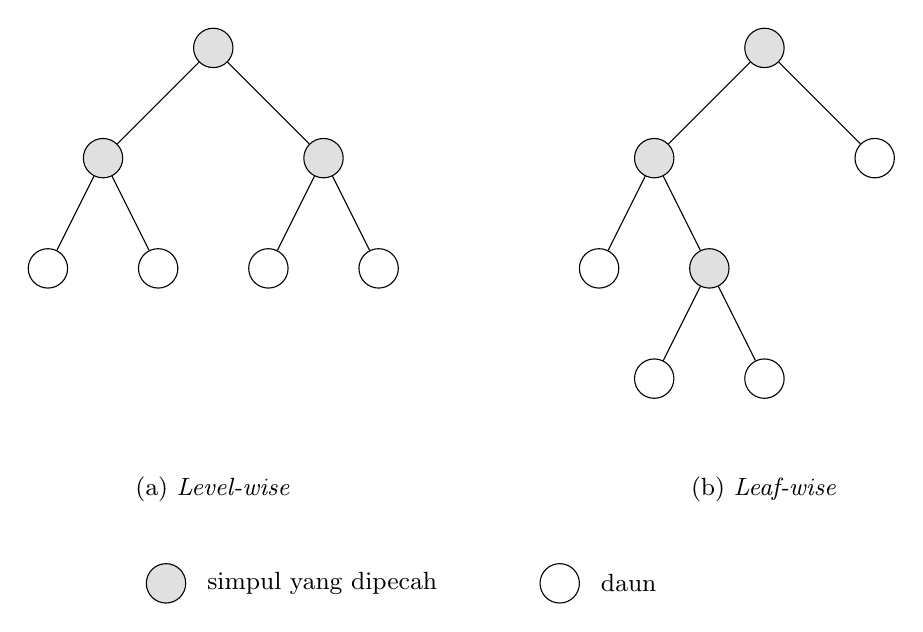
\begin{tikzpicture}[x=1mm,y=-1mm,
      simpul/.style={draw,circle,inner sep=0pt,minimum size=5mm},
      pecah/.style={draw,circle,fill=black!12,inner sep=0pt,minimum size=5mm}]
    % Panel kiri: level-wise
    \begin{scope}
      \node[pecah] (a) at (28,0) {};
      \node[pecah] (b) at (14,14) {};
      \node[pecah] (c) at (42,14) {};
      \node[simpul] (d) at (7,28) {};
      \node[simpul] (e) at (21,28) {};
      \node[simpul] (f) at (35,28) {};
      \node[simpul] (g) at (49,28) {};
      \draw (a) -- (b) (a) -- (c) (b) -- (d) (b) -- (e) (c) -- (f) (c) -- (g);
      \node[font=\small] at (28,56) {(a) \textit{Level-wise}};
    \end{scope}
    % Panel kanan: leaf-wise
    \begin{scope}[xshift=70mm]
      \node[pecah] (a2) at (28,0) {};
      \node[pecah] (b2) at (14,14) {};
      \node[simpul] (c2) at (42,14) {};
      \node[simpul] (d2) at (7,28) {};
      \node[pecah] (e2) at (21,28) {};
      \node[simpul] (f2) at (14,42) {};
      \node[simpul] (g2) at (28,42) {};
      \draw (a2) -- (b2) (a2) -- (c2) (b2) -- (d2) (b2) -- (e2)
            (e2) -- (f2) (e2) -- (g2);
      \node[font=\small] at (28,56) {(b) \textit{Leaf-wise}};
    \end{scope}
    % Legenda di bawah kedua panel.
    \node[pecah] (lg1) at (22,68) {};
    \node[anchor=west,font=\small] at (26,68) {simpul yang dipecah};
    \node[simpul] (lg2) at (72,68) {};
    \node[anchor=west,font=\small] at (76,68) {daun};
  \end{tikzpicture}
  \caption{Pertumbuhan Pohon \textit{Level-wise} dan \textit{Leaf-wise}}
  \label{fig:pohon-lgbm}
  \sumber{Digambar ulang, diadaptasi dari Ke dkk. \cite{ke2017}}
\end{figure}

LightGBM dipilih dengan tiga pertimbangan. Pertama, model berbasis pohon masih
unggul atas \textit{deep learning} pada data tabular berukuran kecil hingga
menengah \cite{grinsztajn2022}, dan data penelitian ini terdiri atas sekitar
3.000 observasi harian. Kedua, akurasinya setara dengan XGBoost
\cite{ke2017,chen2016}, sehingga pilihan di antara keduanya bukan inti
penelitian. Ketiga, sesuai arahan untuk menggunakan ML non-\textit{deep
learning}. Keunggulan kecepatan LightGBM tidak menjadi alasan pemilihan karena
dirancang untuk data besar. Model berbasis pohon juga cenderung meremehkan
volatilitas ekstrem \cite{dudek2024}, sehingga kekalahan model pada hari
lonjakan merupakan kemungkinan yang perlu diantisipasi.

% CEK: Grinsztajn dkk. (2022) dan Chen & Guestrin (2016) belum dicek.

\subsection{Fitur Berbasis Data Intraday}
Selain tiga komponen HAR, penelitian ini menggunakan fitur tambahan (fitur X)
yang seluruhnya diturunkan dari data OHLCV, karena prediktor internal pasar
terbukti paling penting dalam peramalan volatilitas kripto \cite{wang2023}.

\textit{Realized semivariance} negatif mengukur bagian variasi yang berasal
dari \textit{return} negatif \cite{barndorff2010}:
\begin{equation}
  RS_t^- = \sum_{i=1}^{288} r_{t,i}^2 \, \mathbf{1}(r_{t,i} < 0).
  \label{eq:semivarians}
\end{equation}
\begin{keterangan}
  \item[$RS_t^-$] \textit{realized semivariance} negatif pada hari $t$,
  \item[$\mathbf{1}(\cdot)$] fungsi indikator, bernilai 1 bila syarat di
    dalamnya terpenuhi dan 0 bila tidak.
\end{keterangan}
Patton dan Sheppard menunjukkan bahwa \textit{semivariance} negatif lebih
informatif untuk meramal volatilitas pada saham \cite{patton2015}. Karena
$RV_t = RS_t^- + RS_t^+$, fitur yang digunakan adalah proporsi $RS_t^-/RV_t$
agar tidak menimbulkan kolinearitas sempurna dengan komponen HAR.

Estimator \textit{range} Parkinson memanfaatkan harga tertinggi $P^{H}_t$ dan
terendah $P^{L}_t$ dalam satu hari \cite{parkinson1980}:
\begin{equation}
  \sigma^2_{P,t} = \frac{(\ln P^{H}_t - \ln P^{L}_t)^2}{4 \ln 2}.
  \label{eq:parkinson}
\end{equation}
\begin{keterangan}
  \item[$\sigma^2_{P,t}$] estimator varians \textit{range} Parkinson
    pada hari $t$,
  \item[$P^{H}_t$] harga tertinggi pada hari $t$,
  \item[$P^{L}_t$] harga terendah pada hari $t$.
\end{keterangan}
Estimator ini mengasumsikan perdagangan kontinu, asumsi yang lebih terpenuhi
pada Bitcoin yang diperdagangkan 24 jam sehari dibanding saham.

Ukuran \textit{illiquidity} Amihud mengukur dampak harga per satuan volume
transaksi \cite{amihud2002}. Mengikuti Do \cite{do2026}, ukuran ini dihitung
dalam versi \textit{realized} dari bar 5 menit:
\begin{equation}
  \text{Amihud}_t = 10^6 \cdot \frac{1}{N_t}\sum_{i}
  \frac{\left|r_{t,i}\right|}{QV_{t,i}},
  \label{eq:amihud}
\end{equation}
\begin{keterangan}
  \item[$\text{Amihud}_t$] ukuran \textit{illiquidity} pada hari $t$,
  \item[$r_{t,i}$] \textit{return} intraday pada bar ke-$i$,
  \item[$QV_{t,i}$] volume dalam dolar (USDT) pada bar ke-$i$,
  \item[$N_t$] jumlah bar bervolume positif pada hari $t$,
  \item[$10^6$] faktor penskalaan agar besarannya mudah dibaca.
\end{keterangan}
Amihud diperlakukan sebagai proksi dampak harga, bukan
biaya transaksi \cite{amihud2002,brauneis2021}. Fitur lainnya adalah
\textit{return} harian, logaritma volume dolar, dan perubahan logaritma volume.

\subsection{Fungsi Loss untuk Evaluasi Peramalan Volatilitas}
Karena volatilitas sebenarnya tidak teramati, evaluasi peramalan menggunakan
proksi RV. Patton menunjukkan bahwa hanya kelas fungsi \textit{loss} tertentu
yang menghasilkan peringkat model yang konsisten ketika proksi yang digunakan
berisik; dua anggota kelas tersebut adalah MSE dan QLIKE \cite{patton2011}.
Untuk ramalan $F_t$ dan proksi $RV_t$:
\begin{equation}
  L^{\text{QLIKE}}_t = \frac{RV_t}{F_t} - \ln\frac{RV_t}{F_t} - 1,
  \qquad
  L^{\text{MSE}}_t = (RV_t - F_t)^2.
  \label{eq:loss}
\end{equation}
\begin{keterangan}
  \item[$L^{\text{QLIKE}}_t$] nilai \textit{loss} QLIKE pada hari $t$,
  \item[$L^{\text{MSE}}_t$] nilai \textit{loss} MSE pada hari $t$,
  \item[$F_t$] ramalan RV untuk hari $t$,
  \item[$RV_t$] proksi volatilitas teramati pada Persamaan~\ref{eq:rv}.
\end{keterangan}
QLIKE homogen berderajat nol, artinya nilainya tidak berubah bila $RV_t$ dan
$F_t$ dikalikan konstanta yang sama, sehingga \textit{loss} tidak membesar
hanya karena volatilitas sedang tinggi. QLIKE juga menghukum ramalan yang
terlalu rendah lebih berat daripada ramalan yang terlalu tinggi dan memberikan
daya uji yang lebih tinggi \cite{patton2011}. Karena itu QLIKE digunakan sebagai
\textit{loss} utama dan MSE sebagai pelengkap. Ramalan optimal di bawah kedua
\textit{loss} tersebut adalah nilai harapan kondisional \cite{patton2011}.

Objek analisis penelitian ini adalah selisih \textit{loss} harian
\begin{equation}
  \Delta L_t = L_t(\text{ML}) - L_t(\text{HAR}),
  \label{eq:delta-loss}
\end{equation}
\begin{keterangan}
  \item[$\Delta L_t$] selisih \textit{loss} harian antara kedua model,
  \item[$L_t(\text{ML})$] \textit{loss} model \textit{machine learning}
    pada hari $t$,
  \item[$L_t(\text{HAR})$] \textit{loss} model HAR-RV pada hari $t$.
\end{keterangan}
Nilai $\Delta L_t$ yang negatif menunjukkan model ML lebih akurat pada hari
tersebut.
Karena kedua model dievaluasi pada hari dan proksi yang sama, $\Delta L_t$
tidak terpengaruh oleh perubahan skala volatilitas antarperiode.

\subsection{Uji Perbandingan Akurasi Peramalan}
Uji Diebold--Mariano (DM) menguji apakah dua model memiliki akurasi peramalan
yang sama, dengan hipotesis nol $E[\Delta L_t] = 0$ \cite{diebold1995}.
Statistik ujinya adalah
\begin{equation}
  DM = \frac{\overline{\Delta L}}{\sqrt{\widehat{V}_{\text{HAC}} / n}},
  \label{eq:dm}
\end{equation}
\begin{keterangan}
  \item[$DM$] statistik uji Diebold--Mariano,
  \item[$\overline{\Delta L}$] rata-rata selisih \textit{loss} selama
    periode uji,
  \item[$\widehat{V}_{\text{HAC}}$] estimator varians jangka panjang yang
    konsisten terhadap heteroskedastisitas dan autokorelasi,
  \item[$n$] jumlah observasi pada periode uji.
\end{keterangan}
Penelitian ini menggunakan estimator Newey--West \cite{newey1987} dengan \textit{bandwidth}
yang dipilih otomatis menurut Andrews \cite{andrews1991}.

Ketika sejumlah uji dijalankan sekaligus, peluang menemukan hasil signifikan
secara kebetulan meningkat. Prosedur Holm mengendalikan peluang tersebut dengan
mengurutkan \textit{p-value} dan membandingkannya dengan ambang yang makin
longgar secara bertahap \cite{holm1979}. Penelitian ini menetapkan uji
konfirmatori untuk setiap hipotesis sebelum melihat hasil
\textit{out-of-sample}. Hipotesis H2b terdiri atas dua uji sehingga
\textit{p-value}-nya dikoreksi dengan prosedur Holm, sedangkan uji lain
diperlakukan sebagai eksploratori dengan koreksi Holm.

% CEK: Diebold & Mariano (1995) dan Andrews (1991) belum dicek.

\subsection{Instabilitas Kinerja Peramalan dan Uji Perubahan Struktural}
Uji DM membandingkan akurasi rata-rata pada seluruh periode uji. Ketika
lingkungan berubah, kinerja relatif dua model dapat berbeda dari satu
subperiode ke subperiode lain, dan rata-rata keseluruhan dapat menyembunyikan
perubahan tersebut \cite{rossi2013}. Konsep ini perlu dibedakan dari
\textit{forecast breakdown}, yaitu kondisi ketika \textit{loss out-of-sample}
sebuah model secara signifikan lebih buruk daripada \textit{loss in-sample}-nya
\cite{giacomini2009}. Penelitian ini berfokus pada perubahan kinerja
\textbf{relatif} antarmodel, bukan pada kerusakan satu model.

\textit{Fluctuation test} dari Giacomini dan Rossi menghitung statistik DM
secara bergulir pada jendela berukuran $n_F = \mu n$ dan membandingkannya dengan
nilai kritis khusus yang memperhitungkan pengujian berulang
\cite{giacomini2010}. Uji ini menunjukkan kapan satu model lebih unggul, tetapi
hipotesis nolnya adalah kedua model sama akurat di setiap titik waktu, bukan
bahwa kinerja relatifnya stabil. Martins dan Perron menunjukkan bahwa daya uji
\textit{Fluctuation test} rendah dan tidak monoton setelah koreksi HAC, dan
mengusulkan penggunaan uji perubahan struktural pada rata-rata selisih
\textit{loss} \cite{martins2016}.

Uji perubahan struktural Bai--Perron menguji keberadaan perubahan rata-rata
$\Delta L_t$ pada titik waktu yang tidak diketahui \cite{bai1998}. Dengan
$\sup F_T(m)$ adalah statistik \textit{F} terbesar atas semua kemungkinan
penempatan $m$ titik patah, statistik UDmax didefinisikan sebagai
\begin{equation}
  \text{UDmax} = \max_{1 \le m \le M} \sup F_T(m),
  \label{eq:udmax}
\end{equation}
\begin{keterangan}
  \item[$\text{UDmax}$] statistik uji perubahan struktural maksimum,
  \item[$\sup F_T(m)$] statistik $F$ terbesar atas semua kemungkinan
    penempatan $m$ titik patah,
  \item[$M$] jumlah maksimum titik patah yang diuji.
\end{keterangan}
Statistik ini menguji hipotesis nol tanpa perubahan melawan alternatif adanya
satu hingga $M$ perubahan. Setiap segmen dibatasi minimal sebesar proporsi
\textit{trimming} $\varepsilon$ dari sampel. Bai dan Perron menganjurkan UDmax
dijalankan lebih dahulu; bila menolak, jumlah titik patah ditentukan dengan uji
berurutan $\sup F(\ell+1 \mid \ell)$ \cite{bai2003}. Penelitian ini menggunakan
UDmax sebagai uji konfirmatori kestabilan dan \textit{Fluctuation test} sebagai
visualisasi eksploratori.

% CEK: Giacomini & Rossi (2010) baru metadata. Deskripsi mekanisme Fluctuation
% test diambil dari Martins & Perron (2016) dan Rossi (2013) yang sudah full
% text.

\subsection{Evaluasi Out-of-Sample dan Strategi Pembaruan Model}
Evaluasi model peramalan deret waktu harus menghormati urutan waktu. Tashman
menekankan pentingnya evaluasi \textit{out-of-sample} dengan banyak titik asal
peramalan, dan membedakan \textit{updating}, yaitu memasukkan data baru tanpa
mengestimasi ulang parameter, dari \textit{recalibration}, yaitu mengestimasi
ulang parameter dengan data terbaru \cite{tashman2000}. Untuk data yang tidak
stasioner, Cerqueira, Torgo, dan Mozetič merekomendasikan skema
\textit{out-of-sample} berurutan dan validasi \textit{forward-chaining}, bukan
validasi silang acak, karena pengacakan memungkinkan informasi masa depan bocor
ke data latih \cite{cerqueira2020}.

Dalam literatur \textit{concept drift}, cara model beradaptasi terhadap data
yang berubah dikelompokkan antara lain berdasarkan pengelolaan \textit{window}
data latih \cite{gama2014}. \textit{Window} yang tumbuh (\textit{landmark} atau
\textit{expanding}) menyimpan seluruh histori, sedangkan \textit{window} geser
berukuran tetap (\textit{rolling}) hanya memakai data terbaru. Model yang tidak
pernah dilatih ulang berfungsi sebagai pembanding untuk mengukur manfaat
adaptasi \cite{zliobaite2015}. Tabel~\ref{tab:strategi} dan
Gambar~\ref{fig:strategi} merangkum ketiga strategi yang digunakan.

\begin{table}[htbp]
  \caption{Strategi Pembaruan Model dan Padanannya dalam Literatur}
  \label{tab:strategi}
  \centering
  \begingroup
  \setstretch{1}\small
  \begin{tabular}{|c|l|p{0.3\textwidth}|p{0.32\textwidth}|}
    \hline
    \textbf{Kode} & \textbf{Strategi} & \textbf{Data latih} &
    \textbf{Padanan dalam literatur} \\
    \hline
    S0 & Static & Dilatih sekali pada window awal, tidak dilatih ulang &
    \textit{Updating} tanpa rekalibrasi \cite{tashman2000}; pembanding manfaat
    adaptasi \cite{zliobaite2015} \\
    \hline
    S1 & Expanding & Dilatih ulang bulanan dengan seluruh data yang tersedia &
    \textit{Landmark} atau \textit{growing window}
    \cite{gama2014,cerqueira2020} \\
    \hline
    S2 & Rolling & Dilatih ulang bulanan dengan $W$ hari terakhir,
    $W \in \{365, 730\}$; uji konfirmatori memakai $W = 365$ (S2-365) &
    \textit{Fixed-size sliding window} \cite{gama2014} \\
    \hline
  \end{tabular}
  \endgroup
\end{table}

\begin{figure}[htbp]
  \centering
  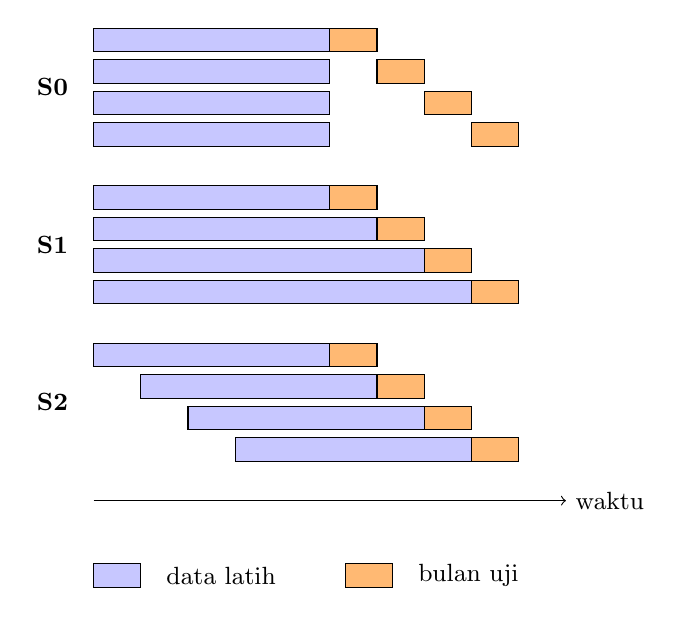
\begin{tikzpicture}[x=1mm,y=-1mm]
    % Sumbu y dibalik (y=-1mm), sehingga posisi baris dihitung langsung di
    % sini; jangan memakai yshift pada scope karena arahnya tidak ikut dibalik.
    \tikzset{
      latih/.style={draw,fill=blue!22},
      uji/.style={draw,fill=orange!55}}
    % Tiga strategi, masing-masing empat iterasi bulanan.
    % S0 baris 0--12, S1 baris 20--32, S2 baris 40--52.
    \foreach \i in {0,...,3} {
      \pgfmathsetmacro\y{\i*4}
      \pgfmathsetmacro\ujix{30+\i*6}
      % S0: data latih tetap pada window awal
      \filldraw[latih] (0,\y) rectangle (30,\y+3);
      \filldraw[uji] (\ujix,\y) rectangle (\ujix+6,\y+3);
      % S1: data latih memanjang dari titik awal
      \filldraw[latih] (0,\y+20) rectangle (\ujix,\y+23);
      \filldraw[uji] (\ujix,\y+20) rectangle (\ujix+6,\y+23);
      % S2: data latih berukuran tetap yang bergeser
      \filldraw[latih] (\i*6,\y+40) rectangle (\i*6+30,\y+43);
      \filldraw[uji] (\ujix,\y+40) rectangle (\ujix+6,\y+43);
    }
    \node[anchor=east,font=\small\bfseries] at (-2,7.5) {S0};
    \node[anchor=east,font=\small\bfseries] at (-2,27.5) {S1};
    \node[anchor=east,font=\small\bfseries] at (-2,47.5) {S2};
    % Sumbu waktu dan legenda
    \draw[->] (0,60) -- (60,60) node[right,font=\small] {waktu};
    \filldraw[latih] (0,68) rectangle (6,71);
    \node[anchor=west,font=\small] at (8,69.5) {data latih};
    \filldraw[uji] (32,68) rectangle (38,71);
    \node[anchor=west,font=\small] at (40,69.5) {bulan uji};
  \end{tikzpicture}
  \caption{Skema Strategi Pembaruan Model Static, Expanding, dan Rolling}
  \label{fig:strategi}
\end{figure}

Pilihan strategi melibatkan \textit{trade-off} bias dan varians. Pesaran dan
Timmermann, sebagaimana dirangkum Rossi, menunjukkan bahwa data sebelum
perubahan struktural menambah bias tetapi mengurangi varians estimasi;
\textit{rolling window} cenderung lebih baik ketika perubahan besar dan
berulang, sedangkan skema rekursif (\textit{expanding}) lebih baik ketika
perubahan kecil \cite{rossi2013}. Untuk model autoregresif seperti HAR, data
sebelum perubahan bahkan dapat mengurangi bias dan varians sekaligus
\cite{rossi2013}. Pilihan \textit{window} pada perbandingan ML dengan HAR juga
harus setara, karena HAR yang diberi skema \textit{fitting} yang kurang tepat
dapat membuat ML tampak unggul secara semu \cite{chassot2026}. Kerangka uji
perbandingan peramalan Giacomini--White dirumuskan untuk skema \textit{rolling}
atau \textit{fixed} \cite{rossi2013}, dan skema \textit{rolling} menyamakan
panjang data latih antarperiode \cite{tashman2000}; karena itu uji formal
kestabilan dijalankan pada skema \textit{rolling}.

\subsection{Pergeseran Distribusi Data}
Pergeseran data (\textit{dataset shift}) terjadi ketika distribusi bersama
masukan dan target pada data uji berbeda dari data latih
\cite{morenotorres2012}. Literatur menggunakan istilah yang berbeda untuk jenis
perubahan yang sama, seperti dirangkum pada Tabel~\ref{tab:istilah}.

\begin{table}[htbp]
  \caption{Perbandingan Istilah Pergeseran Data menurut Gama dkk. dan
    Moreno-Torres dkk.}
  \label{tab:istilah}
  \centering
  \begingroup
  \setstretch{1}\small
  \begin{tabular}{|l|p{0.33\textwidth}|p{0.33\textwidth}|}
    \hline
    \textbf{Perubahan} & \textbf{Gama dkk. \cite{gama2014}} &
    \textbf{Moreno-Torres dkk. \cite{morenotorres2012}} \\
    \hline
    $P(x)$ berubah & \textit{Virtual drift} (tanpa syarat mengenai
    $P(y \mid x)$) & \textit{Covariate shift} (dengan syarat $P(y \mid x)$
    tetap) \\
    \hline
    $P(y \mid x)$ berubah & \textit{Real concept drift} ($P(x)$ boleh berubah) &
    \textit{Concept shift} (dengan syarat $P(x)$ tetap) \\
    \hline
  \end{tabular}
  \endgroup
\end{table}

Peramalan RV termasuk masalah $X \rightarrow Y$, karena fitur hari $t$
mendahului target hari $t+1$, sehingga kerangka Moreno-Torres dkk. yang relevan
\cite{morenotorres2012}. Penelitian ini hanya mengukur perubahan distribusi
fitur $P(x)$ dan tidak menguji apakah $P(y \mid x)$ tetap. Oleh karena itu
istilah yang dipakai adalah \textbf{pergeseran distribusi fitur}, bukan
\textit{covariate shift} atau \textit{concept drift} dalam arti formal.

Pergeseran distribusi satu fitur antara data latih dan bulan uji diukur dengan
statistik Kolmogorov--Smirnov dua sampel,
\begin{equation}
  D^{\text{KS}} = \sup_x
  \left| \hat{F}_{\text{latih}}(x) - \hat{F}_{\text{uji}}(x) \right|,
  \label{eq:ks}
\end{equation}
\begin{keterangan}
  \item[$D^{\text{KS}}$] statistik Kolmogorov--Smirnov dua sampel,
  \item[$\hat{F}_{\text{latih}}(x)$] fungsi distribusi kumulatif empiris
    data latih,
  \item[$\hat{F}_{\text{uji}}(x)$] fungsi distribusi kumulatif empiris
    bulan uji,
  \item[$\sup_x$] nilai terbesar atas seluruh $x$.
\end{keterangan}
Nilai $D^{\text{KS}}$ adalah jarak terbesar antara kedua fungsi distribusi
kumulatif empiris. Uji KS per
fitur merupakan salah satu pendekatan untuk mendeteksi pergeseran data
\cite{rabanser2019}. Nilai $D^{\text{KS}}$ dirata-ratakan antarfitur untuk
memperoleh satu ukuran pergeseran per bulan.

% CEK: Rabanser dkk. (2019) belum dicek.

\subsection{Proksi Likuiditas}
\label{subsec:likuiditas}
Likuiditas pasar kripto dapat diukur dengan berbagai proksi berbasis data harga
dan volume. Brauneis dkk. menunjukkan bahwa proksi yang paling baik menangkap
variasi likuiditas kripto antarwaktu berbeda dengan proksi yang paling baik
menangkap levelnya: estimator \textit{spread} Abdi--Ranaldo unggul untuk
variasi waktu, sedangkan ukuran Amihud unggul untuk level \cite{brauneis2021}.
Karena itu, penelitian ini memakai Amihud sebagai fitur model LGBM-X dan
estimator
Abdi--Ranaldo, yang dihitung dari harga OHLC harian, sebagai variabel likuiditas
dalam analisis asosiasi kinerja relatif dengan kondisi pasar, dengan estimator
Corwin--Schultz sebagai uji sensitivitas. Amihud tidak disertakan pada HAR-X
karena berkolinearitas tinggi dengan komponen HAR berdasarkan pemeriksaan pada
\textit{window} awal; rinciannya diuraikan pada Bab III. Proksi likuiditas harian juga
dipakai Zhang dkk. untuk mengkaji hubungan antara \textit{return} dan
likuiditas aset kripto \cite{zhang2024}.

% CEK: Paper asli estimator Abdi--Ranaldo (2017) dan Corwin--Schultz (2012)
% belum ada di daftar referensi. Tambahkan ke references.bib setelah
% diverifikasi; sementara klaim disandarkan pada Brauneis dkk. (2021).

\section{Kerangka Pemikiran}
Kerangka pemikiran penelitian ini berangkat dari dua fakta. Pertama,
karakteristik pasar Bitcoin berubah lintas era \cite{do2026,mokni2024}. Kedua,
perbandingan model ML dengan HAR-RV umumnya dilaporkan sebagai satu hasil
agregat \cite{dudek2024,huang2024}, padahal kinerja relatif dapat berubah
sepanjang waktu \cite{rossi2013,gama2014}. Dari kedua fakta tersebut,
penelitian ini menanyakan apakah kinerja relatif LightGBM terhadap HAR-RV
stabil, faktor pasar apa yang berasosiasi dengan perubahannya, dan bagaimana
strategi pembaruan model memengaruhinya.

Untuk menjawabnya, perbedaan kinerja diurai melalui desain $2 \times 2$ pada
Tabel~\ref{tab:desain}. Perbandingan LGBM-HAR dengan HAR mengukur kontribusi
non-linearitas, perbandingan HAR-X dengan HAR mengukur kontribusi informasi
tambahan, dan perbandingan LGBM-X dengan HAR mengukur kontribusi total. Model
\textit{naive persistence} ($\widehat{RV}_{t+1} = RV_t$) disertakan sebagai
pemeriksaan kewajaran \cite{gama2014}.

\begin{table}[htbp]
  \caption{Desain Perbandingan Model $2 \times 2$}
  \label{tab:desain}
  \centering
  \begingroup
  \setstretch{1}
  \begin{tabular}{|l|c|c|}
    \hline
    & \textbf{Masukan HAR} & \textbf{Masukan HAR + fitur X} \\
    \hline
    \textbf{Linear} & HAR-RV (pembanding) & HAR-X \\
    \hline
    \textbf{Non-linear} & LGBM-HAR & LGBM-X \\
    \hline
  \end{tabular}
  \endgroup
\end{table}

Pada HAR-X, fitur X tidak mencakup ukuran Amihud (lihat
Subbab~\ref{subsec:likuiditas}).

Alur kerangka pemikiran ditunjukkan pada Gambar~\ref{fig:kerangka}.

\begin{figure}[htbp]
  \centering
  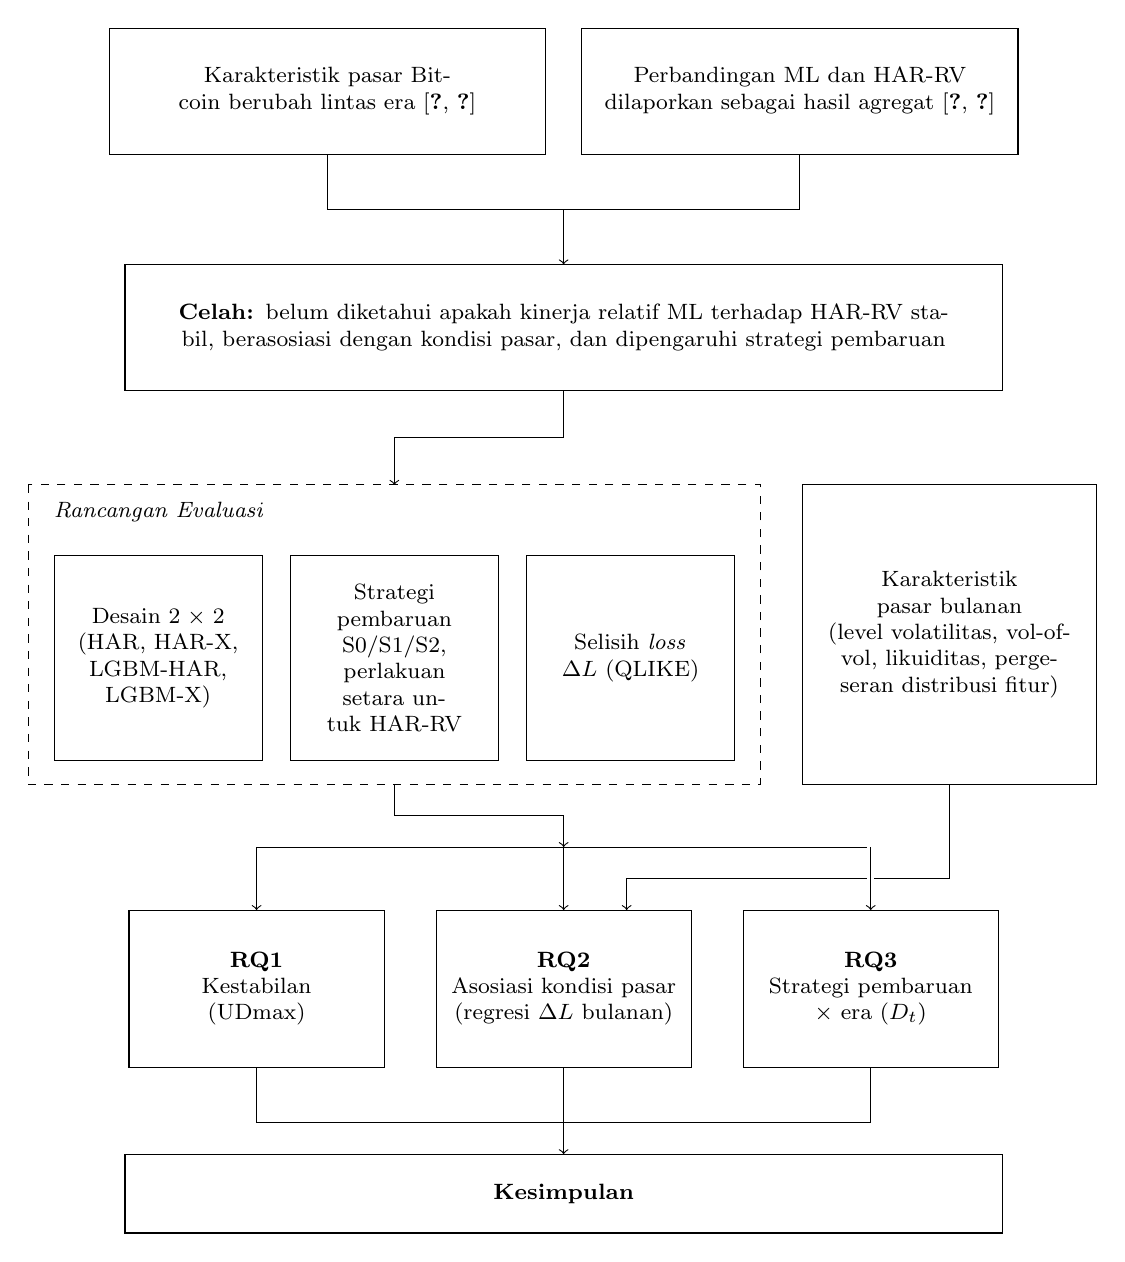
\begin{tikzpicture}[x=1mm,y=-1mm,
      kotak/.style={draw,align=center,inner sep=2pt,font=\footnotesize},
      fakta/.style={kotak,text width=54mm,minimum height=16mm},
      lebar/.style={kotak,text width=110mm},
      komponen/.style={kotak,text width=25mm,minimum height=26mm},
      pasar/.style={kotak,text width=36mm,minimum height=38mm},
      rq/.style={kotak,text width=31mm,minimum height=20mm}]

    % --- Baris 1: dua fakta pembuka yang berdiri sejajar ---------------------
    \node[fakta] (faktaa) at (-30,0)
      {Karakteristik pasar Bitcoin berubah lintas era
       \cite{do2026,mokni2024}};
    \node[fakta] (faktab) at (30,0)
      {Perbandingan ML dan HAR-RV dilaporkan sebagai hasil agregat
       \cite{dudek2024,huang2024}};

    % --- Baris 2: celah tempat kedua fakta bertemu ---------------------------
    \node[lebar,minimum height=16mm] (celah) at (0,30)
      {\textbf{Celah:} belum diketahui apakah kinerja relatif ML terhadap
       HAR-RV stabil, berasosiasi dengan kondisi pasar, dan dipengaruhi
       strategi pembaruan};

    % --- Baris 3: wadah rancangan evaluasi dan masukan karakteristik pasar ---
    \draw[dashed] (-68,50) rectangle (25,88);
    \node[anchor=north west,font=\footnotesize\itshape] at (-66,51)
      {Rancangan Evaluasi};
    \node[komponen] at (-51.5,72)
      {Desain $2 \times 2$\\(HAR, HAR-X,\\LGBM-HAR, LGBM-X)};
    \node[komponen] at (-21.5,72)
      {Strategi pembaruan\\S0/S1/S2, perlakuan\\setara untuk HAR-RV};
    \node[komponen] at (8.5,72)
      {Selisih \textit{loss}\\$\Delta L$ (QLIKE)};
    \node[pasar] (pasar) at (49,69)
      {Karakteristik pasar bulanan\\(level volatilitas, vol-of-vol,
       likuiditas, pergeseran distribusi fitur)};

    % --- Baris 4: tiga rumusan masalah --------------------------------------
    \node[rq] (rq1) at (-39,114) {\textbf{RQ1}\\Kestabilan\\(UDmax)};
    \node[rq] (rq2) at (0,114)
      {\textbf{RQ2}\\Asosiasi kondisi pasar\\(regresi $\Delta L$ bulanan)};
    \node[rq] (rq3) at (39,114)
      {\textbf{RQ3}\\Strategi pembaruan\\$\times$ era ($D_t$)};

    % --- Baris 5: kesimpulan, sengaja generik karena bab ini pra-hasil ------
    \node[lebar,minimum height=10mm] (simpulan) at (0,140) {\textbf{Kesimpulan}};

    % --- Panah --------------------------------------------------------------
    % Kedua fakta bertemu di satu titik sebelum masuk ke kotak celah.
    \draw (-30,8) -- (-30,15);
    \draw (30,8) -- (30,15);
    \draw (-30,15) -- (30,15);
    \draw[->] (0,15) -- (0,22);
    % Celah mengarah ke wadah rancangan evaluasi.
    \draw (0,38) -- (0,44) -- (-21.5,44);
    \draw[->] (-21.5,44) -- (-21.5,50);
    % Satu panah dari wadah ke baris RQ, lalu dibagikan ke ketiga kotak.
    \draw (-21.5,88) -- (-21.5,92) -- (0,92);
    \draw[->] (0,92) -- (0,96);
    \draw (-39,96) -- (39,96);
    \draw[->] (-39,96) -- (-39,104);
    \draw[->] (0,96) -- (0,104);
    % Karakteristik pasar hanya memberi masukan ke RQ2.
    \draw[->] (49,88) -- (49,100) -- (8,100) -- (8,104);
    % Digambar terakhir dengan halo putih agar tampak melompati garis di atas.
    \draw[white,line width=2.4pt] (39,96) -- (39,104);
    \draw[->] (39,96) -- (39,104);
    % Ketiga RQ bermuara pada satu kesimpulan.
    \draw (-39,124) -- (-39,131);
    \draw (0,124) -- (0,131);
    \draw (39,124) -- (39,131);
    \draw (-39,131) -- (39,131);
    \draw[->] (0,131) -- (0,135);
  \end{tikzpicture}
  \caption{Kerangka Pemikiran Penelitian}
  \label{fig:kerangka}
\end{figure}

\section{Hipotesis Penelitian}
Berdasarkan landasan teori di atas, hipotesis penelitian dirumuskan sebagai
berikut.

\textbf{H1.} Rata-rata selisih \textit{loss}
$\Delta L(\text{LGBM-X} - \text{HAR})$ tidak konstan sepanjang periode
pengujian. Hipotesis ini diturunkan dari perubahan karakteristik pasar Bitcoin
lintas era \cite{do2026,mokni2024} dan dari literatur instabilitas peramalan
\cite{rossi2013,martins2016}.

\textbf{H2a.} Selisih \textit{loss} bulanan berasosiasi dengan sedikitnya satu
karakteristik pasar, yaitu level volatilitas, volatilitas dari volatilitas,
likuiditas, atau pergeseran distribusi fitur. Pendekatan meregresikan ukuran
kinerja peramalan pada indikator yang teramati mengikuti semangat Giacomini dan
Rossi \cite{giacomini2009}.

\textbf{H2b.} Kontribusi fitur X terhadap kinerja relatif berbeda antara era
\textit{transition} dan \textit{institutional}. Do menunjukkan bahwa hubungan
volatilitas--likuiditas berubah antarera \cite{do2026}, tetapi Do menguji arah
volatilitas terhadap \textit{illiquidity}, sedangkan penelitian ini memakai
likuiditas dan volume untuk meramal RV; H2b merupakan perluasan dari temuan
tersebut. Mokni dkk. menunjukkan hubungan likuiditas dapat berbalik tanda
\cite{mokni2024}, dan kepentingan fitur tidak konsisten antarstudi
\cite{wang2023,feng2024ml}. Karena itu H2b dirumuskan dua arah.

\textbf{H3.} Pada era \textit{institutional}, kinerja relatif LGBM-X terhadap
HAR-RV lebih baik pada strategi \textit{rolling} 365 hari (S2-365)
dibandingkan \textit{expanding} (S1). Dengan
$D_t = \Delta L_t(\text{S2-365}) - \Delta L_t(\text{S1})$, dan $\Delta L_t$
adalah selisih \textit{loss} LGBM-X terhadap HAR-RV pada
Persamaan~\ref{eq:delta-loss}, H3 didukung bila rata-rata $D_t$ negatif dan
signifikan. Hipotesis ini
didasarkan pada \textit{trade-off} bias--varians \cite{rossi2013} dan perubahan
persistensi RV antarera \cite{do2026}: hubungan yang dipelajari dari era awal
dapat usang, dan LGBM-X yang lebih fleksibel diduga lebih terdampak data usang
daripada HAR.

\textbf{Hipotesis tandingan.} Hasil yang berlawanan dengan H3 tetap bermakna.
Untuk model autoregresif, data sebelum perubahan struktural dapat mengurangi
bias dan varians sekaligus, sehingga skema \textit{expanding} dapat lebih baik
daripada \textit{rolling} \cite{rossi2013}. Selain itu, bila \textit{regime}
volatilitas berulang, data lama tetap relevan \cite{gama2014,suarez2023}.

Ringkasan rumusan masalah, hipotesis, dan uji konfirmatorinya disajikan pada
Tabel~\ref{tab:ringkasan}. Uji konfirmatori ditetapkan sebelum hasil
\textit{out-of-sample} dilihat.

\begin{table}[htbp]
  \caption{Ringkasan Rumusan Masalah, Hipotesis, dan Uji Konfirmatori}
  \label{tab:ringkasan}
  \centering
  \begingroup
  \setstretch{1}\small
  \begin{tabular}{|p{0.22\textwidth}|c|p{0.47\textwidth}|}
    \hline
    \textbf{Rumusan masalah} & \textbf{Hipotesis} &
    \textbf{Uji konfirmatori} \\
    \hline
    RQ1 Kestabilan kinerja relatif & H1 &
    UDmax pada rata-rata $\Delta L(\text{LGBM-X} - \text{HAR})$, skema rolling
    365 hari, QLIKE, HAC, $\varepsilon = 0{,}15$, maksimum 5 perubahan; bila
    tidak menolak, uji DM pada seluruh sampel \\
    \hline
    RQ2 Asosiasi dengan kondisi pasar & H2a, H2b &
    H2a: uji-F bersama (HAC) pada regresi $\Delta L$ bulanan terhadap
    4 karakteristik pasar. H2b: dua uji-t HAC beda rata-rata antara era
    \textit{transition} dan \textit{institutional}, untuk
    $\Delta L(\text{HAR-X} - \text{HAR})$ dan
    $\Delta L(\text{LGBM-X} - \text{LGBM-HAR})$, dengan koreksi Holm \\
    \hline
    RQ3 Strategi pembaruan $\times$ era & H3 &
    Uji-t HAC dua sisi pada rata-rata
    $D_t = \Delta L_t(\text{S2-365}) - \Delta L_t(\text{S1})$ pasangan LGBM-X
    dan HAR-RV di era \textit{institutional} \\
    \hline
  \end{tabular}
  \endgroup
\end{table}
